\documentclass{article}
\usepackage{physics}
\usepackage{graphicx}
\usepackage{caption}
\usepackage{amsmath}
\usepackage{bm}
\usepackage{framed}
\usepackage{authblk}
\usepackage{empheq}
\usepackage{amsfonts}
\usepackage{esint}
\usepackage[makeroom]{cancel}
\usepackage{dsfont}
\usepackage{centernot}
\usepackage{mathtools}
\usepackage{subcaption}
\usepackage{bigints}
\usepackage{amsthm}
\theoremstyle{definition}
\newtheorem{lemma}{Lemma}
\newtheorem{defn}{Definition}[section]
\newtheorem{prop}{Proposition}[section]
\newtheorem{rmk}{Remark}[section]
\newtheorem{thm}{Theorem}[section]
\newtheorem{exmp}{Example}[section]
\newtheorem{prob}{Problem}[section]
\newtheorem{sln}{Solution}[section]
\newtheorem*{prob*}{Problem}
\newtheorem{exer}{Exercise}[section]
\newtheorem*{exer*}{Exercise}
\newtheorem*{sln*}{Solution}
\usepackage{empheq}
\usepackage{tensor}
\usepackage{xcolor}
%\definecolor{colby}{rgb}{0.0, 0.0, 0.5}
\definecolor{MIT}{RGB}{163, 31, 52}
\usepackage[pdftex]{hyperref}
%\hypersetup{colorlinks,urlcolor=colby}
\hypersetup{colorlinks,linkcolor={MIT},citecolor={MIT},urlcolor={MIT}}  
\usepackage[left=1in,right=1in,top=1in,bottom=1in]{geometry}

\usepackage{newpxtext,newpxmath}
\newcommand*\widefbox[1]{\fbox{\hspace{2em}#1\hspace{2em}}}

\newcommand{\p}{\partial}
\newcommand{\R}{\mathbb{R}}
\newcommand{\C}{\mathbb{C}}
\newcommand{\lag}{\mathcal{L}}
\newcommand{\nn}{\nonumber}
\newcommand{\ham}{\mathcal{H}}
\newcommand{\M}{\mathcal{M}}
\newcommand{\I}{\mathcal{I}}
\newcommand{\K}{\mathcal{K}}
\newcommand{\F}{\mathcal{F}}
\newcommand{\w}{\omega}
\newcommand{\lam}{\lambda}
\newcommand{\al}{\alpha}
\newcommand{\be}{\beta}
\newcommand{\x}{\xi}

\newcommand{\G}{\mathcal{G}}

\newcommand{\f}[2]{\frac{#1}{#2}}

\newcommand{\ift}{\infty}

\newcommand{\lp}{\left(}
\newcommand{\rp}{\right)}

\newcommand{\lb}{\left[}
\newcommand{\rb}{\right]}

\newcommand{\lc}{\left\{}
\newcommand{\rc}{\right\}}


\newcommand{\V}{\mathbf{V}}
\newcommand{\U}{\mathcal{U}}
\newcommand{\Id}{\mathcal{I}}
\newcommand{\D}{\mathcal{D}}
\newcommand{\Z}{\mathcal{Z}}

%\setcounter{chapter}{-1}


\usepackage{enumitem}



\usepackage{listings}
\captionsetup[lstlisting]{margin=0cm,format=hang,font=small,format=plain,labelfont={bf,up},textfont={it}}
\renewcommand*{\lstlistingname}{Code \textcolor{violet}{\textsl{Mathematica}}}
\definecolor{gris245}{RGB}{245,245,245}
\definecolor{olive}{RGB}{50,140,50}
\definecolor{brun}{RGB}{175,100,80}

%\hypersetup{colorlinks,urlcolor=colby}
\lstset{
	tabsize=4,
	frame=single,
	language=mathematica,
	basicstyle=\scriptsize\ttfamily,
	keywordstyle=\color{black},
	backgroundcolor=\color{gris245},
	commentstyle=\color{gray},
	showstringspaces=false,
	emph={
		r1,
		r2,
		epsilon,epsilon_,
		Newton,Newton_
	},emphstyle={\color{olive}},
	emph={[2]
		L,
		CouleurCourbe,
		PotentielEffectif,
		IdCourbe,
		Courbe
	},emphstyle={[2]\color{blue}},
	emph={[3]r,r_,n,n_},emphstyle={[3]\color{magenta}}
}


\begin{document}
\begin{framed}
\noindent Name: \textbf{Huan Q. Bui}\\
Course: \textbf{8.422 - AMO II}\\
Problem set: \textbf{\#4}\\
Due: Friday, Mar 10, 2022\\
References: 
\end{framed}
	
	
\noindent \textbf{1. Squeezing Hamiltonian.} \\

\noindent The dimensionless squeezing Hamiltonian is 
\begin{align*}
\ham = \f{\hbar \omega}{2} (\tilde{p}^2 - \tilde{x}^2). 
\end{align*}
With $p = (\tilde{p}- \tilde{x}) / \sqrt{2}$ and $x = (\tilde{p} + \tilde{x})/\sqrt{2}$, we have $[x,p] = \tilde{x}, \tilde{p} = i$ and the Hamiltonian becomes
\begin{align*}
\ham = \hbar \omega xp
\end{align*}
plus an offset which we ignore. 

\begin{enumerate}[label=(\alph*)]

\item Let $\psi_0(x)$ be given. In the spirit on the question, we will simply plug $\psi_0(x(t))$ into the Schr\"{o}dinger equation as a test solution and see what happens:
\begin{align*}
i\hbar \f{\p}{\p t} \psi_0(x(t)) &= \hbar \omega x p \psi_0(x(t))  \\
i \psi_0'(x(t)) x'(t) &= -i \omega  x(t)t \psi_0'(x(t)) \\
x'(t) &= - \omega x(t),
\end{align*}
where we have used $p = -i\p_x$. We see that we could arrive this same differential equation for $x(t)$ irrespective of the functional form of $\psi_0(x)$, so we may conclude that $\psi(x,t) = \psi_0(x(t))$. The equation for $x(t)$ is:
\begin{align*}
x(t) = x_0 e^{-\omega t}. 
\end{align*}




\item Let $\tilde{\psi}_0(p)$ be given. Before calculating more, let us modify our Hamiltonian so that the operators are in a "good" order. By adding a constant term $-i\hbar \omega$ to $H$ (just like what we did in the beginning) to get 
\begin{align*}
H \to \hbar\omega xp - i\hbar\omega = \hbar\omega px,
\end{align*}
without changing the dynamics.  With $x = i \p/\p p$ in momentum space we calculate, similar to Part (a):
\begin{align*}
i\hbar \f{\p}{\p t} \tilde{\psi}_0(p(t)) &= i \hbar \omega p(t) \f{\p}{\p p}  \tilde{\psi}_0(p(t))  \\
\tilde{\psi}_0'(p(t)) p'(t) &=  \omega p(t)\tilde{\psi}_0'(p(t))   \\
p'(t) &= \omega p(t).
\end{align*}
From here, we find $p(t)$:
\begin{align*}
p(t) = p_0 e^{\omega t}.
\end{align*}

\item Suppose $\psi_0(x) = e^{-x^2/2} / \pi^{1/4}$, which is the wavefunction of the vacuum in the $x$-representation. This wavefunction has width $1/\sqrt{2}$. At a time $t$, space is rescaled by a factor $e^{-\omega t}$ and acquires an extra factor of $e^{-\omega t/2}$ in order to maintain normalization. In any case, because $x \to x e^{-\omega t}$, the new wavefunction is 
\begin{align*}
\psi_0(x)= \f{e^{-\omega t/2}}{\pi^{1/4}} \exp\lb -\f{1}{2} x^2 e^{-2\omega t}  \rb. 
\end{align*}
We can just read off from here that the new width $\Delta x$ becomes $e^{\omega t}$ times the original width of $1/\sqrt{2}$. 


\item By a similar argument to that in Part (c), the new wavefunction in momentum space acquires an extra factor for $e^{\omega t/2}$ to maintain normalization. Because $p \to p e^{\omega t}$, we see that the new width $\Delta p$ is now $e^{-\omega t}$ times the original width of $1/\sqrt{2}$.

\item From Parts (c) and (d), we see quite easily that $\Delta x \Delta p = e^{\omega t - \omega t}/2 = 1/2$, which is the same as the uncertain at $t=0$, as expected. 

\item Here we rewrite the Hamiltonian in proper symmetrized form:
\begin{align*}
H = \f{\hbar \omega}{2} (xp + px).
\end{align*} 
With $a = (x+ip)/\sqrt{2}$ and $a^\dagger = (x - ip)/\sqrt{2}$, we find 
\begin{align*}
H 
&= \f{\hbar \omega}{2} \lb \f{a + a^\dagger}{\sqrt{2}} \f{ a - a^\dagger }{\sqrt{2} i} + \f{a - a^\dagger}{\sqrt{2} i} \f{a+a^\dagger}{\sqrt{2}} \rb \\
&= \f{\hbar \omega}{4i} (  a^2 - aa^\dagger + a^\dagger a - {a^\dagger}^2+ a^2 + aa^\dagger - a^\dagger a -  {a^\dagger}^2 ) \\
&= \f{\hbar \omega}{2i} (a^2 - {a^\dagger}^2).
\end{align*}

We find the familiar Hamiltonian that appeared in lecture. 

\end{enumerate}



\noindent \textbf{2. Disentangling the Squeezing Operator.} \\

\noindent In this problem we show that
\begin{align*}
e^{\f{r}{2} ( {a^\dagger}^2 - a^2)}  \ket{0} = \f{1}{\sqrt{\cosh r}} \sum_{n=0}^\infty  \f{\sqrt{(2n)!}}{2^n n!} (\tanh r)^n \ket{2n}.
\end{align*}
To do this, we follow the parts below. 

\begin{enumerate}[label=(\alph*)]

\item We first calculate the following commutators:
\begin{align*}
[a^2, {a^\dagger}^2] 
&=   aa a^\dagger a^\dagger - a^\dagger a^\dagger a a \\
&= a(1+a^\dagger a) a^\dagger - a^\dagger (aa^\dagger - 1) a \\
&= 1 + a^\dagger a + (1+a^\dagger a)(1 + a^\dagger a ) - a^\dagger a a^\dagger a + a^\dagger a \\
&= 4a^\dagger a + 2. 
\end{align*}
\begin{align*}
[a^2, a^\dagger a ] 
&= aaa^\dagger a - a^\dagger a a a  \\
&= a(1+a^\dagger a) a - (aa^\dagger -1) aa \\
&= 2a^2.
\end{align*}
\begin{align*}
[{a^\dagger}^2 , a^\dagger a] 
&= a^\dagger a^\dagger a^\dagger a  - a^\dagger a a^\dagger a^\dagger \\
&= a^\dagger a^\dagger (aa^\dagger - 1) - a^\dagger (1 + a^\dagger a) a^\dagger \\
&= -2{a^\dagger}^2.
\end{align*}

From these, we conclude that the Lie algebra of operators $\{  a^2, {a^\dagger}^2, a^\dagger a + 1/2  \}$ is closed under commutation. This means we must be able to write
\begin{align*}
e^{\f{r}{2} ({a^\dagger}^2 - a^2)  } = e^{\f{u}{2} {a^\dagger}^2} e^{t(^\dagger a + 1/2)} e^{\f{v}{2}a^2}. 
\end{align*}
Our job now is to find the numbers $u,t,v$, which are functions of $r$. To do this, we find any other Lie algebra whose three operators obey the same commutation relations which allows us to more easily find $u,t,v$. It turns out that Pauli matrices work. 

\item Consider the replacement:
\begin{align*}
a^\dagger a + \f{1}{2} 
&\to \sigma_z = 
\begin{pmatrix}
1 & 0 \\ 0 & -1 
\end{pmatrix} \\
a^2 
&\to -\sigma_- 
= -\sigma_x +  i\sigma_y 
= 
\begin{pmatrix}
0 & 0 \\ -2 & 0
\end{pmatrix} \\
{a^\dagger}^2
&\to \sigma_+ = \sigma_x + i\sigma_y = 
\begin{pmatrix}
0 & 2 \\ 0 & 0
\end{pmatrix}
\end{align*}
Let us check that the commutation relations above still hold. 
\begin{align*}
[a^2, {a^\dagger}^2]
\to
[-\sigma_-, \sigma_+] 
=
[-\sigma_x, i\sigma_y]  + [i\sigma_y, \sigma_x] = 4\sigma_z \leftarrow 4a^\dagger a + \f{1}{2}  \quad \checkmark
\end{align*}
\begin{align*}
[a^2, a^\dagger a] 
\to 
[-\sigma_-, \sigma_z - 1/2] = [-\sigma_-, \sigma_z] 
= 
2i\sigma_y -2\sigma_x = 2(-\sigma_-) \leftarrow 2 a^2 \quad \checkmark
\end{align*}
\begin{align*}
[{a^\dagger}^2, a^\dagger a] 
=
[\sigma_+, \sigma_z - 1/2] = [\sigma_+, \sigma_z]
=
-2i\sigma_y -2 \sigma_x = -2 \sigma_+  \leftarrow  -2 {a^\dagger}^2 \quad \checkmark
\end{align*}


\item With
\begin{align*}
\f{r}{2}\lp {a^\dagger}^2 - a^2 \rp = \f{r}{2}(\sigma_+  + \sigma_-) = r\sigma_x = \begin{pmatrix}
0 & r \\ r& 0
\end{pmatrix},
\end{align*}
we find 
\begin{align*}
e^{\f{r}{2}\lp {a^\dagger}^2 - a^2 \rp } = \begin{pmatrix}
\cosh r & \sinh r \\ \sinh r & \cosh r
\end{pmatrix}.
\end{align*}
Mathematica code:
\begin{lstlisting}
In[7]:= MatrixExp[r*PauliMatrix[1]] // FullSimplify
Out[7]= {{Cosh[r], Sinh[r]}, {Sinh[r], Cosh[r]}}
\end{lstlisting}


\item Similarly, we have
\begin{align*}
U = e^{\f{u}{2} {a^\dagger}^2} = \exp\lb \f{u}{2} \begin{pmatrix}  
0 & 2 \\ 0 & 0 
\end{pmatrix} \rb = 
\exp\lb \begin{pmatrix}  
0 & u \\ 0 & 0 
\end{pmatrix} \rb 
= \begin{pmatrix}
1 & u \\ 0 & 1
\end{pmatrix}
\end{align*}
\begin{align*}
T = e^{t\lp a^\dagger a + 1/2 \rp} = e^{t\sigma_z} = \exp\lb \begin{pmatrix} t & 0 \\ 0 & -t  \end{pmatrix} \rb
= \begin{pmatrix}
e^t & 0 \\ 0 & e^{-t}
\end{pmatrix}
\end{align*}
\begin{align*}
V = e^{\f{v}{2}a^2} = \exp\lb \f{v}{2}\begin{pmatrix}  0 & 0 \\ -2 & 0   \end{pmatrix} \rb
= \exp\lb \begin{pmatrix}  0 & 0 \\ -v & 0  \end{pmatrix} \rb = \begin{pmatrix}
1 & 0 \\ -v & 1
\end{pmatrix}.
\end{align*}
With these,
\begin{align*}
UTV = 
\begin{pmatrix}
e^t - e^{-t} uv & e^{-t} u    \\ -e^{-t} v & e^{-t}
\end{pmatrix}.
\end{align*}
Mathematica code:
\begin{lstlisting}
In[14]:= U = MatrixExp[{{0, u}, {0, 0}}]
Out[14]= {{1, u}, {0, 1}}

In[15]:= T = MatrixExp[t*PauliMatrix[3]]
Out[15]= {{E^t, 0}, {0, E^-t}}

In[16]:= V = MatrixExp[{{0, 0}, {-v, 0}}]
Out[16]= {{1, 0}, {-v, 1}}

In[18]:= U . T . V // FullSimplify
Out[18]= {{E^t - E^-t u v, E^-t u}, {-E^-t v, E^-t}}
\end{lstlisting}

\item Comparing the results of Parts (c) and (d) we easily find that
\begin{align*}
t = -\ln \cosh r, \quad\quad u = -v = e^t \sinh r = \tanh r .
\end{align*}
so we have
\begin{align*}
e^{\f{r}{2}\lp {a^\dagger}^2 - a^2 \rp} = e^{\f{\tanh r }{2} {a^\dagger}^2} e^{-\ln \cosh r  \lp a^\dagger a + 1/2 \rp} e^{-\f{\tanh r }{2} a^2} = 
\f{1}{\sqrt{\cosh r}} 
e^{\f{\tanh r }{2} {a^\dagger}^2} e^{-\ln \cosh r  ( a^\dagger a ) } e^{-\f{\tanh r }{2} a^2}
\end{align*}


\item Applying the operator above to $\ket{0}$, we realize that the two right most operators act on $\ket{0}$ as the identity, so we end up with
\begin{align*}
e^{\f{r}{2}\lp {a^\dagger}^2 - a^2 \rp} \ket{0} 
&= \f{1}{\sqrt{\cosh r}} e^{\f{\tanh r }{2} {a^\dagger}^2}  \ket{0} \\
&= \f{1}{\sqrt{\cosh r}} \sum_{n=0}^\infty  \f{(\tanh r)^n}{2^n n!} {a^\dagger}^{2n}  \ket{0} \\
&= \f{1}{\sqrt{\cosh r}} \sum_{n=0}^\infty \f{\sqrt{(2n)!}}{2^n n!} (\tanh r)^{n} \ket{2n},
\end{align*}
as desired. 

\end{enumerate}



\noindent \textbf{3. Generation of Squeezed States by Two-Photon Interactions.}\\


\noindent Consider a mode $(\vec{k}, \vec{\epsilon})$ with wavevector $\vec{k}$ and polarization $\vec{\epsilon}$ of the EM field with frequency $\omega$ whose Hamiltonian is given by 
\begin{align*}
H = \hbar \omega a^\dagger a + i\hbar \Lambda \lb (a^\dagger)^2 e^{-2i\omega t} - a^2 e^{2i \omega t } \rb.
\end{align*}
The first term is the energy of the mode of the free field. The second term describes a
two-photon interaction process such as parametric amplification (a classical wave of frequency $2\omega$
generating two photons with frequency $\omega$). $\Lambda$ is a real quantity characterizing the strength of the interaction. In this problem, we will show that this Hamiltonian produces squeezed vacuum and explore how
it acts on coherent states.

\begin{enumerate}[label=(\alph*)]

\item The equation of motion for $a(t)$ in the Heisenberg picture is 
\begin{align*}
\f{d}{dt}a_H = \f{i}{\hbar} [H_H, a_H],
\end{align*}
where the Hamiltonian in the Heisenberg picture is simply the Schr\"{o}dinger equation but in terms of $a_H$ and $a_H^\dagger$:
\begin{align*}
H_H =  \hbar \omega a_H^\dagger a_H + i\hbar \Lambda \lb (a_H^\dagger)^2 e^{-2i\omega t}  - a_H^2 e^{2i\omega t} \rb.
\end{align*}


Now we compute the commutators:
\begin{align*}
[a^\dagger a , a] = -[a,a^\dagger a] = -[a,a^\dagger] a - a^\dagger [a,a] = -a.
\end{align*}
\begin{align*}
[(a^\dagger)^2, a] = -[a,(a^\dagger)^2] = -[a,a^\dagger]a^\dagger - a^\dagger [a, a^\dagger] = -2a^\dagger
\end{align*}
 \begin{align*}
 [a^2,a] = 0
\end{align*}
From these, we find the equations of motion for $a$ and $a^\dagger$
\begin{align*}
\dot a
&=  -i \omega a + 2 \Lambda a^\dagger  e^{-2i\omega t} \\
\dot a^\dagger
&= i \omega a^\dagger + 2\Lambda a  e^{2i\omega t}
\end{align*}
In matrix form:
\begin{align*}
\begin{pmatrix} 
\dot a \\ \dot a^\dagger
\end{pmatrix}
=
\begin{pmatrix}
-i\omega & 2\Lambda e^{-2\omega t} \\ 2\Lambda e^{2i\omega t} & i \omega 
\end{pmatrix}
\begin{pmatrix}
a \\ a^\dagger
\end{pmatrix}.
\end{align*}

To solve this, we consider the ansatz $a(t) = b(t)e^{-i\omega t}$. After we plug in this substitution, the system of equations above becomes:
\begin{align*}
\dot{b}(t) e^{-i\omega t} = 2\Lambda b^\dagger(t) e^{-2i\omega t + i\omega t} \implies \dot{b}(t) = 2\Lambda b^\dagger(t) \implies \dot{b}^\dagger(t) = 2\Lambda b(t).
\end{align*}
From here, we find the equations of motion for $b(t)$ and $b^\dagger(t)$: 
\begin{align*}
\ddot{b}(t) = 4\Lambda^2 b(t) \quad\quad \text{and} \quad\quad \ddot{b}^\dagger(t) = 4\Lambda^2 b^\dagger(t).
\end{align*}



\item The contribution of the mode $(\vec{k}, \vec{\epsilon})$ to the electric field is 
\begin{align*}
\vec{E}(\vec{r},t) = i\mathcal{E}_\omega \vec{\epsilon} \lb a(t) e^{i\vec{k}\cdot \vec{r}} - a^\dagger(t) e^{-i \vec{k} \cdot \vec{r}} \rb
\end{align*}
where $a(t) = b(t) e^{-i\omega t}$.  Consider the quantities
\begin{align*}
b_P(t) = \f{b(t) + b^\dagger(t)}{2} \quad\quad \text{and} \quad\quad  b_Q(t) = \f{b(t) -b^\dagger(t)}{2i}.
\end{align*}
We now show that they represent physically two quadrature components of the field. To this end, we simply plug in expression for $a(t)$ in terms of $b(t)$ and expand the electric field in terms of trigonometric functions:
\begin{align*}
\vec{E}(\vec{r},t) 
&= i\mathcal{E}_\omega \vec{\epsilon} \lb  b(t) e^{i (\vec{k}\cdot \vec{r} -  \omega t)}  - b^\dagger(t) e^{-i(\vec{k}\cdot \vec{r} - \omega t)}   \rb \\ 
&= i\mathcal{E}_\omega \vec{\epsilon} \lb [b(t) - b^\dagger(t)] \cos(\vec{k}\cdot \vec{r} - \omega t) + i[b(t) + b^\dagger(t)] \sin(\vec{k}\cdot \vec{r} - \omega t)   \rb \\ 
&= -2\mathcal{E}_\omega \vec{\epsilon} \lb   b_Q(t) \cos(\vec{k}\cdot \vec{r} - \omega t)  +  b_P(t) \sin(\vec{k}\cdot \vec{r} - \omega t)  \rb.
\end{align*}
So we see that $b_P(t)$ and $b_Q(t)$ represent the two quadrature components of the electric field, as desired. Since $b_P(t)$ and $b_Q(t)$ are linear superpositions of $b(t)$ and $b^\dagger(t)$, $b_Q(t)$ and $b_P(t)$ also solve the similar differential equation as $b(t)$ and $b^\dagger(t)$:
\begin{align*}
\ddot{b}_P(t) = 4\Lambda^2 b_P(t) \quad\quad \text{and} \quad\quad \ddot{b}_Q(t) = 4\Lambda^2 b_Q(t),
\end{align*}
where $b_P(t)$ and $b_Q(t)$ are uncoupled, unlike $b(t)$ and $b^\dagger(t)$. Let us now solve for $b_P(t), b_Q(t), b(t), b^\dagger(t)$ in terms of $b(0)$ and $b^\dagger(0)$. From its differential equation we find the general form for $b(t)$ and $b^\dagger(t)$:
\begin{align*}
b(t)               &= c_1 e^{2\Lambda t} + c_2 e^{-2\Lambda t} \implies b(0) = c_1 + c_2\\
b^\dagger(t) &= c_1 e^{2\Lambda t} - c_2 e^{-2\Lambda t} \implies b^\dagger(0) = c_1 - c_2.
\end{align*}
From $b_P(0)$ and $b_Q(0)$ we can solve for $c_1, c_2$:
\begin{align*}
c_1 =  b_P(0) \quad\quad \text{and} \quad\quad c_2 = ib_Q(0).
\end{align*}
And we're done:
\begin{align*}
b(t) &= b_P(0) e^{2\Lambda t} + ib_Q(0) e^{-2\Lambda t} 
= \f{b(0) + b^\dagger(0)}{2} e^{2\Lambda t} + \f{b(0) - b^\dagger(0)}{2} e^{-2\Lambda t} \\ 
b^\dagger(t) &= b_P(0) e^{2\Lambda t} - ib_Q(0) e^{-2\Lambda t} 
= \f{b(0) + b^\dagger(0)}{2} e^{2\Lambda t} - \f{b(0) - b^\dagger(0)}{2} e^{-2\Lambda t} \\ 
b_P(t) &= b_P(0)  e^{2\Lambda t}   \\
b_Q(t) &= b_Q(0) e^{-2\Lambda t}.
\end{align*}


\item Assume that at time $t=0$ the electromagnetic field is in the vacuum state. Then at time $t$:
\begin{align*}
\langle N \rangle_t 
&= \bra{0}  a^\dagger(t) a(t) \ket{0} \\
&= \bra{0}  b^\dagger(t) b(t) \ket{0} \\
&= \bra{0} \lp  \f{b +b^\dagger}{2} e^{2\Lambda t} - \f{b -b^\dagger}{2} e^{-2\Lambda t} \rp 
 \lp  \f{b +b^\dagger}{2} e^{2\Lambda t} + \f{b -b^\dagger}{2} e^{-2\Lambda t} \rp \ket{0} \\
 &= \bra{0} \lp  \f{a +a^\dagger}{2} e^{2\Lambda t} - \f{a -a^\dagger}{2} e^{-2\Lambda t} \rp 
 \lp  \f{a +a^\dagger}{2} e^{2\Lambda t} + \f{a -a^\dagger}{2} e^{-2\Lambda t} \rp \ket{0} \\ 
 &= \f{e^{4\Lambda t}}{4} + \f{e^{-4\Lambda t}}{4} - \f{1}{2} \\
 &= \f{1}{2}( \cosh(4\Lambda t) - 1 ).
\end{align*}
Here we have used $a = a(0) = b(0)$ and $a^\dagger = a^\dagger(0) = b^\dagger(0)$.  We notice that the average number of photon increases exponentially as a function of $t$. 


Next we compute,
\begin{align*}
\bra{0}  b_P(t)   \ket{0} 
&= \f{e^{2\Lambda t}}{2} \bra{0} a + a^\dagger  \ket{0} = 0 \\
\bra{0} b_Q(t) \ket{0} 
&= \f{e^{-2\Lambda t}}{2} \bra{0}   a - a^\dagger \ket{0} = 0\\
\bra{0}   b_P(t)^2  \ket{0} 
&=  \f{e^{4\Lambda t}}{4} \bra{0} (a + a^\dagger)^2 \ket{0} = \f{e^{4\Lambda t}}{4} \\ 
\bra{0} b_Q(t)^2 \ket{0}
&= -\f{e^{-4\Lambda t}}{4} \bra{0} (a - a^\dagger)^2 \ket{0} = \f{e^{-4\Lambda t}}{4}.
\end{align*}
With these we find the dispersions:
\begin{align*}
\Delta b_P(t) = \f{e^{2\Lambda t}}{2} \quad\quad \text{and} \quad\quad \Delta b_Q(t) = \f{e^{-2\Lambda t}}{2}.
\end{align*}
We clearly see that there is squeezing: one quadrature grows while the other decays exponentially. However, $\Delta b_P(t) \Delta b_Q(t) = 1/2$ for all times $t$, as it should be due to Heisenberg. 




\item In class, we defined the squeezed vacuum with parameter $z = re^{i\phi}$ as
\begin{align*}
\ket{0_z} = S(z)\ket{0} = \exp\lb \f{1}{2}z^* a^2 -\f{1}{2} z{a^\dagger}^2 \rb \ket{0} = 
\f{1}{\sqrt{\cosh r}} \sum_{n=0}^\infty \f{\sqrt{(2n)!}}{2^n n!}( \tanh r)^n e^{i 2n \phi } \ket{2n}.
\end{align*}
We will now show that the two-photon interaction Hamiltonian above produces this state and this operator when we apply it for a time $t_0$. \\

Since the free field part of the Hamiltonian $\hbar \omega a^\dagger a$ annihilates the vacuum state $\ket{0}$, we can simply ignore it. This leaves us with only the two-photon part. The time evolution operator is then given by 
\begin{align*}
e^{iHt_0/\hbar} 
&= \exp\lb \Lambda \lp {a(t_0)^2 e^{2i\omega t_0 } -  a^\dagger (t_0)}^2 e^{-2i \omega t_0 } \rp \rb \\
&= \exp\lb \Lambda e^{2i\omega t_0 }  a(t_0)^2 -   \Lambda e^{-2i \omega t_0 }  {a^\dagger(t_0)}^2  \rb \\
&=  \exp\lb \Lambda   b(t_0)^2 -   \Lambda   {b^\dagger(t_0)}^2  \rb \\ 
&= \exp\lb \Lambda   b(t_0)^2 -   \Lambda   {b^\dagger(t_0)}^2  \rb.
\end{align*}
Now we compute $b(t_0)^2 - b^\dagger(t_0)$:
\begin{align*}
b(t_0)^2 - b^\dagger(t_0)^2
&= \f{1}{4}\lb  (b + b^\dagger) e^{2\Lambda t_0} +(b- b^\dagger) e^{-2\Lambda t_0} \rb^2
-\f{1}{4}  \lb  (b + b^\dagger) e^{2\Lambda t_0} - (b- b^\dagger) e^{-2\Lambda t_0} \rb^2\\
&= \f{1}{4}\lb 2 (b+b^\dagger)(b - b^\dagger) + 2 (b-b^\dagger)(b+b^\dagger) \rb \\ 
&= \f{1}{2}\lb bb-bb^\dagger + b^\dagger b - b^\dagger b^\dagger + b^2 + bb^\dagger - b^\dagger b - b^\dagger b^\dagger \rb \\ 
&= b^2  - {b^\dagger}^2.
\end{align*}
 So, we have
 \begin{align*}
 e^{i Ht_0/\hbar} = \exp\lb \Lambda b^2 - \Lambda {b^\dagger}^2  \rb.
 \end{align*}
 By identifying this with the squeezing operator $S(z) = \exp[z^* b^2/2 - z{b^\dagger}^2/2]$, we find that $z = 2\Lambda$. We have derived the resulting state in Problem 2, so there is no need to do that again here. We notice that there is no dependence on $t_0$. 


\item In order to plot the follow $Q$ distributions we must calculate the amplitudes. 

\begin{itemize}

\item $Q_1(\al)$ is for the squeezed vacuum $S(z) \ket{0}$:
\begin{align*}
Q_1(\al) = \abs{\bra{\al} S(z) \ket{0}}^2 = \abs{\f{e^{-\abs{\al}^2/2}}{\sqrt{\cosh |z|}} \sum_{n=0}^\infty \f{(\al^*)^{2n}}{2^n n!} (\tanh |z|)^n}^2.
\end{align*}

\begin{figure}[!htb]
	\centering
	\begin{minipage}{.3\textwidth}
  	\centering
  	\includegraphics[width=.55\linewidth]{figures/Q1-z-02.eps}
  	\captionof{figure}{$z = 0.2$}
	\end{minipage}%
	\begin{minipage}{.3\textwidth}
  	\centering
  	\includegraphics[width=.55\linewidth]{figures/Q1-z-12.eps}
  	\captionof{figure}{$z = 1.2$}
	\end{minipage}
	\begin{minipage}{.3\textwidth}
  	\centering
  	\includegraphics[width=.55\linewidth]{figures/Q1-z-40.eps}
  	\captionof{figure}{$z = 4.0$}
	\end{minipage}
\end{figure} 



\item Displaced squeezed state $Q_2(\al)$:
\begin{align*}
Q_2(\al) = \abs{ \bra{\al } D(\be) S(z) \ket{0} }^2 = 
\abs{\f{e^{-\abs{\al - \be}^2/2}}{\sqrt{\cosh |z|}} \sum_{n=0}^\infty \f{(\al^* - \be^*)^{2n}}{2^n n!} (\tanh |z|)^n}^2.
\end{align*}
where we have used $\bra{\al} D(\be) = \bra{\al} D^\dagger(-\be) = \bra{\al - \be}$. For this and the next part of the problem let us choose $\be = 2$. 


\begin{figure}[!htb]
	\centering
	\begin{minipage}{.3\textwidth}
  	\centering
  	\includegraphics[width=.55\linewidth]{figures/Q2-z-02.eps}
  	\captionof{figure}{$z = 0.2$}
	\end{minipage}%
	\begin{minipage}{.3\textwidth}
  	\centering
  	\includegraphics[width=.55\linewidth]{figures/Q2-z-12.eps}
  	\captionof{figure}{$z = 1.2$}
	\end{minipage}
	\begin{minipage}{.3\textwidth}
  	\centering
  	\includegraphics[width=.55\linewidth]{figures/Q2-z-40.eps}
  	\captionof{figure}{$z = 4.0$}
	\end{minipage}
\end{figure} 

\item A squeezed coherent state $Q_3(\al)$:
\begin{align*}
Q_3(\al) 
&= \abs{ \bra{\al } S(z) D(\be) \ket{0} }^2 = \abs{ \bra{\al}  D(\be_-) S(z) \ket{0} }^2 \\
&= \abs{ \bra{\al}  D(\be \cosh z - \be^* \sinh z ) S(z) \ket{0} }^2 \\
&= 
\abs{\f{e^{-\abs{\al - \be \cosh z + \be^* \sinh z }^2/2}}{\sqrt{\cosh |z|}} \sum_{n=0}^\infty \f{(\al^* - \be^* \cosh^* z + \be \sinh^* z )^{2n}}{2^n n!} (\tanh |z|)^n}^2.
\end{align*}

\begin{figure}[!htb]
	\centering
	\begin{minipage}{.3\textwidth}
  	\centering
  	\includegraphics[width=.55\linewidth]{figures/Q3-z-02.eps}
  	\captionof{figure}{$z = 0.2$}
	\end{minipage}%
	\begin{minipage}{.3\textwidth}
  	\centering
  	\includegraphics[width=.55\linewidth]{figures/Q3-z-12.eps}
  	\captionof{figure}{$z = 1.2$}
	\end{minipage}
	\begin{minipage}{.3\textwidth}
  	\centering
  	\includegraphics[width=.55\linewidth]{figures/Q3-z-40.eps}
  	\captionof{figure}{$z = 4.0$}
	\end{minipage}
\end{figure} 

\end{itemize}


Looking at $Q_2$ and $Q_3$, we see that they behave very similarly, except for the rate at which the peak of the $Q$-distribution gets displaced as a function of $z$. This makes sense, as this rate is determined by the hyperbolic trigonometric functions of $z$ for $Q_3$. What's interesting is that the squeezed coherent state is NOT the same as the displaced squeezed vacuum. \\

By thinking about how the time evolution of the $Q$-distribution reflects on the measurement of the electric field, we can see that the two-photon interaction generates phase squeezing. 


\end{enumerate}






\end{document}








